\documentclass[a4paper]{article}
\usepackage{afterpage}
\usepackage{caption}
\usepackage{subcaption}
\usepackage{hanging}
\usepackage{setspace}
\usepackage[a4paper, margin=1.2in]{geometry}
\usepackage[
backend=biber,
style=chem-biochem,
citestyle=nature,
url=false,
doi=true,
isbn=false,
autocite=superscript
]{biblatex}
\usepackage{todonotes}
\usepackage{doi}
\usepackage{titlesec}
\usepackage{hyperref}
\usepackage{caption}
\usepackage{subcaption}
\usepackage{pdflscape}

\renewcommand{\thefootnote}{\alph{footnote}}
\newcommand{\sectionbreak}{\clearpage}
\renewcommand*{\bibfont}{\footnotesize}
\addbibresource{../../references.bib}
\bibliographystyle{unsrtnat}
\urlstyle{rm}

\hypersetup{
    colorlinks=true,
    citecolor=magenta,
    linkcolor=magenta
}

\setlength{\parskip}{0.75em}

\onehalfspacing

\pagestyle{plain}

\graphicspath{ {./figures/} }

\renewcommand{\abstractname}{Summary}

\title{
	{\normalsize Doctoral Thesis Proposasal} \\
	{\LARGE \textsc{Building Resilience: How do Species Interactions Shape Ecosystem Collapse?}}
}
\author{
  {\large Fernando Cagua}
}
\date{}

\begin{document}

\maketitle

\begin{abstract}
  Natural ecosystems provide important services---like food and water---we humans depend on to a large extent.
  Much like the failure of a single key financial institution can trigger unexpected crashes on the stock market, human pressures---such as biological invasions and species extinctions---can cause sudden collapses that severely transform the way ecosystems function.
  However, despite its importance, we do not completely understand the dynamics that make ecosystems resilient to collapse.
  Because the functioning of ecosystems is largely determined by the network of interactions between the species that inhabit them, my proposed research aims to quantify the role played by species interactions in determining the resilience of ecosystems.
  To achieve this, I will focus on networks of mutually beneficial interactions, like those between plants and their pollinators, and use a combination of empirical data, computer simulations and ecological theory.
  Ultimately I want to understand why, when and how ecosystem collapses occur, and how to recover from them.
\end{abstract}









\section*{Introduction}
\addcontentsline{toc}{section}{Introduction}

From food and freshwater production, to recreation and carbon sequestration, ecosystems provide a wide range of services of considerable value to humans.
Unfortunately, the frequency of undesired ecosystem collapses---like the (often sudden) shift from a transparent to a turbid lake or from a self-sustaining fishery to a collapsed one---is dramatically increasing worldwide\autocite{Scheffer2001a}.
When ecosystem resilience is limited, breakdowns are more likely, and their ability to provide those services we depend on is endangered.
Therefore, a necessary step to anticipate, prevent, and reverse ecosystem collapse is to understand the processes that support or undermine ecosystem resilience \autocite{Hughes2005, Tylianakis2008}.

Resilience is related to the amount of disturbance that an ecosystem could withstand without collapsing, or, in ecological jargon, undergoing a regime shift---a large, persistent transformation in ecosystem functioning and structure \autocite{Holling1973, Gunderson2000}.
Moreover, substantial research indicates that ecosystem functioning and structure are largely determined by the network of interactions formed by species in an ecological community \autocite{Bascompte2006, Dobson2006, Tylianakis2008, Reiss2009}.
Since these factors ultimately determine the ecosystem response to disturbances, \textbf{the overall objective of my proposed research is to quantify the role played by species interactions in modulating ecosystem resilience}.

To do so, I will focus on the network of mutualistic interactions between plants and pollinators \autocite{Bascompte2006, Bascompte2007, Klein2007}.
These networks, which form the base of pollination systems, play a globally important role in the maintenance of biodiversity and crop production \autocite{Bascompte2007, Klein2007}.
Pollination systems are locally important too; for instance two thirds of New Zealand plants are pollinated by birds or insects\autocite{Cox2000}, and this includes iconic native plants (like k\={o}whai and p\={o}hutukawa), and economically important crops (like kiwifruit, apples and grapes). However, pollination systems worldwide are currently being disrupted by multiple drivers of human-driven global change \autocite{Cox2000}.

Pollination is being affected particularly affected by the simultaneous loss of previously important species, and the introduction of invasive species.
My thesis will concentrate on the resistance and resilience of pollination systems to biotic invasions and defaunation---top components of human-caused global change.
These two drivers have affected New Zealand with particular intensity; at the same time, it remains notably vulnerable \autocite{Vitousek1997}.
For instance, 50\% of plant species in New Zealand are introduced \autocite{Wilton2000}, and imported social bees are now an important component of pollinator fauna \autocite{Lloyd1985, Newstrom2005}.
Moreover, the depletion of native birds \autocite{Anderson2003, Robertson2009} is a prime example of how pollination systems in New Zealand are losing key pollinators, plants and habitats\autocite{Cox2000}.

Empirical, time continuous observations of ecosystem dynamics in networks that have been subjected to invasions are limited.
Therefore, I will focus on empirically informed theoretical approaches.
Throughout my thesis, I will use computer simulated communities to estimate the population dynamics of the species in the community, and then I will directly quantify stability properties from fluctuations in the species populations \autocite{Bastolla2009, Garcia-Algarra2013}.
I will develop these `sinthetic` communities under a wide range of parameters to answer the specific questions I aim to answer in each chapter of my dissertation.

In the first chapter of my thesis I will concentrate on biotic invasions.
Specifically I have a twofold objective: \textbf{first, I aim to determine which network characteristics shape the its resistance and resilience to invasions}, and second \textbf{to determine how biotic invasions, by affecting existing interactions in the community, reshape network resistance and resilience}.
Answering this question requires a deep understanding of the requirements for stable species coexistence in ecological communities.
Therefore I will simulate communities with different network structures, and analyze which structures are more favorable for the coexistence of the invasive species.
I will then in turn, see how the structure itself is changed by the invasive species, and whether the change in structure has stability implications.

Remarkably, invaded pollination communities have been shown to have structures that support more species \autocite{Stouffer2014} and can be more robust than those of un-invaded communities \autocite{Albrecht2014}.
Indeed we know which structures can enhance biodiversity \autocite{Bastolla2009} and delay the onset of catastrophic collapses \autocite{Lever2014}, but there are still serious mismatches between theoretical predictions and empirical observations.
I argue that this can be at least partially explained by the interplay between the degree of redundancy among species in the network and the apparent facilitation and competition between species in a mutualistic network.
Therefore, the objective of my second chapter is to \textbf{evaluate the effects of that structural redundancy has on the stability of ecological networks}.
For that I will use measures of local and global redundancy and quantify the relationship between these metrics (in synthetic and empirical communities) and the stability of the community.

The first two chapters of my thesis are designed to answer underlying questions of resilience theory, however the underlying aim of my third chapter is to translate the gained insight into useful lessons for ecosystem management.
Ecosystems are complex, non-linear systems that are very difficult to control.
However, recent work in theoretical physics has highlighted that is indeed possible to regulate them using targeted interventions \autocite{Cornelius2013}.
I propose to build upon these findings to \textbf{determine the optimal set of management actions---from both a theoretical and a feasibility perspective---that are required to modify an ecosystem state}.
A previous study has collected empirical data to characterized the network of interactions before and after an ecological invasion \autocite{Bartomeus2008}.
First, I will use that dataset to find the set of species that can act as drivers of ecosystem state.
Then, I will focus on an extension of the population models that serve as backbone of my dissertation.
I aim to determine the characteristics---like the degree of generalization of trophic position---that make an species more likely to serve as a driver of ecosystem state.
Rescuing ecosystems from the brink of collapse and recovering them from undesired shifts is a major goal in conservation science.
Finding a way in which actions targeted to specific species can maximize the ecosystem resilience, will bring us much closer to that goal.

In a world of constant change, building resilience is our best insurance against losing the ecosystem services we value and depend on.
Although we have identified some of the pervasive effects of invasions and defaunation at the species level, we currently do not understand how the changes on ecosystem dynamics is affecting the resilience of the ecosystems as a whole.
The research I propose intends to establish the general theory necessary to answer this question.
Doing so is especially important when the ecosystem response might be inconspicuous until transformation is imminent.
Only by better understanding the dynamics behind species interactions, can we hopefully be better prepared to anticipate, prevent and reverse undesired ecosystem collapses.









\section{Ecosystems stability to species invasions} \label{chapter1}

The invasion of naturalized species is changing ecosystems worldwide.
Fortunately, during the last four decades, there has been steady progress in understanding the causes and outcomes of biotic invasions.
For instance, we now understand that the success of an ecological invasion depends on geographic, bio-climatic, and taxonomic factors, as well as aspects of reproductive biology and general ecology of the introduced organisms.
However, we are still unable to successfully predict the outcome of species introductions in a large proportion of cases.

One of the potential explanations for this limited predictive success is that research on both the causes and consequences of invasive species, have focused on the negative interactions between species in the community (competition, and predator-prey relationships).
However the establishment of an introduced species depends on, or at least is greatly enhanced, by the establishment of  mutualistic relationships \autocite{Richardson2000}---in which both interacting species have a positive outcome.
In fact, there are multiple empirical examples of plants that only become successful invaders, when mutualistic partners that pollinate their flowers, or disperse their seeds, are available \autocite{Simberloff1999, Simberloff2006, Prior2014}.
Understanding the reciprocal relationship between biotic invasions and mutualism is a key step necessary to both improving current predictions of invasion outcomes, as well as evaluating how invasive species are modifying mutualistic systems \autocite{Richardson2000}.

\subsection{Species coexistence theory underpins the invasibility of ecosystems}

It has been recently shown that there exists a direct link between the structure of ecological networks and ecosystem stability \autocite{Bascompte2006,Rooney2006,Okuyama2008,Bastolla2009, Tylianakis2010, Thebault2010,Rohr2014,Sauve2014}.
In particular stable species coexistence in mutualistic networks seems to be favoured by highly diverse, connected, and nested structures \autocite{Okuyama2008, Bastolla2009, Thebault2010, Sauve2014}.
For instance, the nested structure observed in many mutualistic networks---in which specialist species tend to interact with a subset of the species with which a generalist interact---support higher amounts of biodiversity, minimises competition among species in the community and maximises the range of conditions necessary to have a stable community \autocite{Bastolla2009, Rohr2014}.
The unambiguous link between ecosystem stability and the ecosystem response to disturbances is an important argument for investigating the implications of network structure and its vulnerability to drivers of global change.

Perturbations caused by global change are severely modifying the structure of mutualistic networks \autocite{Burkle2013a}.
Indeed, current evidence suggests that most of its effects are negative \autocite{Tylianakis2008, Tylianakis2010}.
Although our understanding of the effects of those perturbations is limited, we know that, for instance, climate change, and habitat modification can lead to shifts on species abundances, and mismatches of phenology, behaviour, or geographic ranges of the interacting species \autocite{Memmott2007, Tylianakis2008, Hegland2009, Burkle2013a}.
Those changes can in turn disrupt the patterns of interactions that determine the structure of mutualistic networks.
Some evidence suggest other factors of global change like biotic invasions can also modify the structure of mutualistic networks, for example through changes in the strength of species interactions, and the degree of network nestedness and connectivity \autocite{Olesen2002, Aizen2008, Bartomeus2008, Vila2009, Traveset2013}

I hypothesise that network structure is not only modified by the succesive invasion of alien species, but it also plays an important role in determining the invasibility of the community.
Two facts provide support to this hypothesis.
First, mutualistic interactions are key for the invasion success of introduced species because introduced species need to have suitable pollinators in the new habitat in order to establish themselves in the community \autocite{Richardson2000, Sargent2008}.
Second, the structure of mutualistic interactions is known to have direct implications for the number of coexisting species in the community \autocite{Moeller2004, Bascompte2006, Bascompte2007, Bastolla2009}.
Specifically, structures that minimise plant competition seem to facilitate species coexistence and promote biodiversity \autocite{Bastolla2009}.
Therefore structural attributes---like the degree of specialisation/generalisation, and the contribution to nestedness, of available pollinators---should influence the likelihood an introduced species becomes invasive \autocite{Stouffer2014}.

Previous studies have have found that simpler networks, with fewer species and fewer interactions between species, are easier to invade \autocite{Romanuk2009, Galiana2014}.
However, these studies are strictly limited to trophic networks in which interactions are chiefly antagonistic (prey-predator) \autocite{Romanuk2009, Baiser2010, Galiana2014}.
Unfortunately, these results cannot be easily extrapolated because mutualistic interactions introduce facilitative and competitive feedbacks that are not present in antagonistic interactions.
Here I will fill that gap, and study the link between different structural attributes of mutualistic networks---degree of nestedness, contribution to nestedness, and compartmentalisation.

The first step to achieve that is to construct simulated communities of mutualistic interactions.
The structure of those communities will be determined by implementing the varying structure of empirically observed networks, as well as by constructing simulated networks with a wide range of structural parameters (\autoref{fig:networks}).
This will allow me to evaluate if the network structures that have been found to minimise competition also make the community more vulnerable to invasions.

\begin{figure}[tbp]
  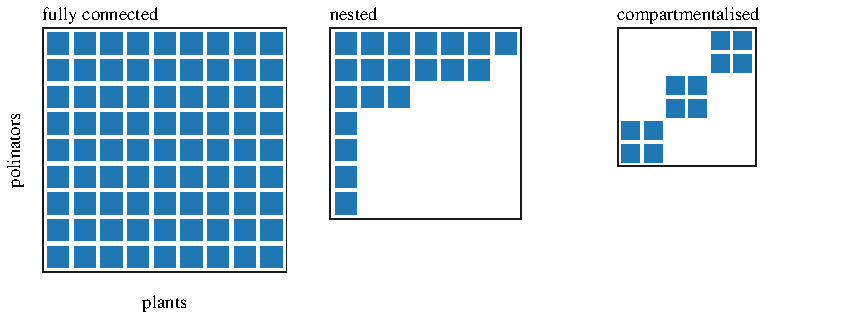
\includegraphics{networks}
  \caption{
  \label{fig:networks}
  Each panel represents a plant–animal network with different network structures.
  Plants compete for resources such as nutrients, but also have indirect interactions mediated by their common pollinators.
  As the number of shared pollinators is higher, positive effects outweigh negative one.
  Current theory predicts a higher number of coexisting species as indicated by the size of the matrices.
  }
\end{figure}

The second step is to develop models of the population dynamics in mutualistic communities in which the abundances of each species present on the community depends on their growth rate ($births - deaths$).
These growth rates can in turn be affected by the feedbacks imposed by the interactions with other species.
In this model, there is competition between species that belong to the same group (plants or pollinators), while facilitation ocurs between species that belong to different groups.
Specifically I will use a recently introduced logistic model that is mathematically simpler but preserves the dynamic richness of previous models \autocite{Garcia-Algarra2013}.
Like in previous studies using dynamic models \autocite{Okuyama2008, Bastolla2009}, I will assume that the beneficial effect of mutualistic partners saturates at high abundances.

The third step is to analyse the ecosystem response to an alien species.
Depending on the network structure, and the traits of the native and alien species, the outcome of an species introduction can vary.
One possible outcome option is that alien species is not able to invade the community(\hyperref[fig:dynamics]{Figure \ref{fig:dynamics}a}).
Another possibility is that the alien species becomes an invader, which can, in some instances, have catastrophic consequences for other species in the community (\hyperref[fig:dynamics]{Figure \ref{fig:dynamics}b, c}).
respond.
Therefore, I will quantify the invasibility of the community as the likelihood that an invader is successful \autocite{Ives2007, Romanuk2009}.

\begin{figure}[tbp]
  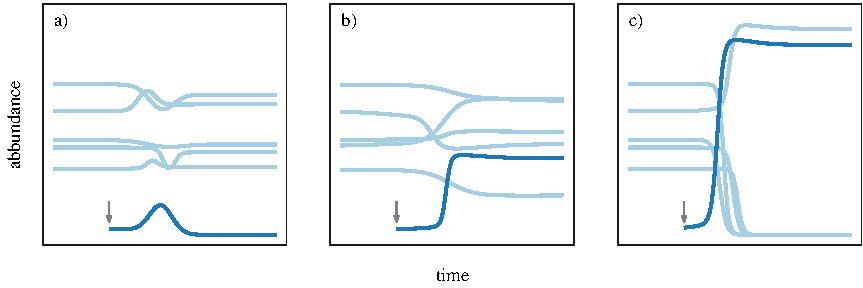
\includegraphics{dynamics}
  \caption{
  \label{fig:dynamics}
  Three possible responses of ecosystems in stable coexistence to the introduction of an alien species (dark blue):
  (a) the alien species did not succeed to coexist, and caused only minor changes in the abundances of the species already present in the community (light blue);
  (b) the alien species persisted with the original species; or
  (c) the alien species became invasive, and five of the original species went extinct.
  }
\end{figure}

Because, as mentioned, a nested structure maximises the number of species that can stably coexist \autocite{Bastolla2009}, I predict that a similar relationship exists between invasibility and nestedness (\hyperref[fig:hypo_c1]{Figure \ref{fig:hypo_c1}a}).
Additionally because a compartmentalised structure, might limit the potential for apparent facilitation between the native and invasive species I argue that there is a neggative relationship between invasibility and compartmentalisation (\hyperref[fig:hypo_c1]{Figure \ref{fig:hypo_c1}b}).
This hypotheses link concepts of network structure, apparent competition/facilitation and ecosystem stability, and will allow us to put limited and somewhat disparate empirical observations in context.

\begin{figure}[p]
  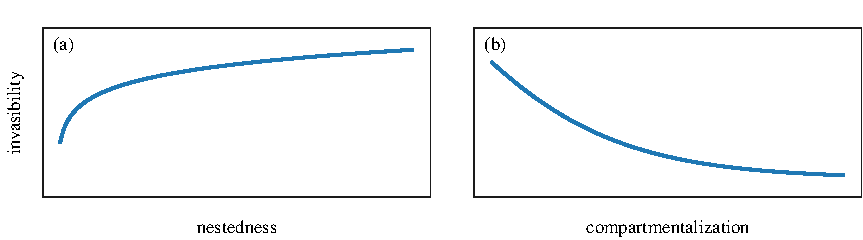
\includegraphics{hypo_c1}
  \caption{
  \label{fig:hypo_c1}
  It has been found that (a) an increasingly nested structure enhances the number of species that can stable coexist, while (b) a compartmentalized structure decreases it.
  I hypothesise that a similar relationship exist between these attributes of network structure and the invasibility of the community.
  }
\end{figure}

Despite the general belief that successful invasive species tend to be super-generalists \autocite{Richardson2000, Aizen2008, Vila2009, Albrecht2014}, a recent meta-analysis has shown that invasive species become very integrated in pollination networks \autocite{Stouffer2014}.
Specifically, invasive plants seem to interact preferentially with pollinators that are weak contributors to community nestedness, which have been shown to be the less vulnerable to extinction \autocite{Saavedra2011, Stouffer2014}.
However this empirical observation has not yet been explained mechanistically.
By testing the hypotheses I propose, not only will light be shed on what makes ecosystem vulnerable to invasions, but also, because they deal with fundamental tenets in theoretical ecology, we will also gain a better understanding of the implications of network structure on the persistence of biodiversity, the link between stability and biodiversity, and the assembly of ecological communities.

\subsection{Invasions change the structure of mutualistic networks}

After analyising the structures that make an ecological network more or less susceptible to invasions, I then follow by investigating the consequences for the community when the invasion is successful (\autoref{fig:diagram_c1}).
On one hand, I will explore the feedbacks on the structure of mutualistic network after an successful invasion; on the other hand I will explore when the invasions lead to a large number of secondary extinctions and ultimately ecosystem collapse (\hyperref[fig:dynamics]{Figure \ref{fig:dynamics}c}).

\begin{figure}[p]
  \centering
  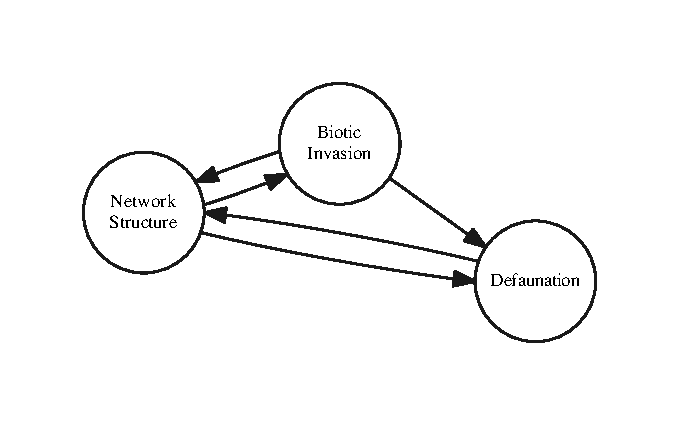
\includegraphics{diagram_c1}
  \caption{
  \label{fig:diagram_c1}
  The network structure determines the invasibility of an ecological community.
  However, successful invasions also modify the structure itself, whether trough a shift in interaction partners or trough secondary extinctions in the community.
  }
\end{figure}

Successful invasive species have been shown to have pollination effects in the native species trough changes on pollinator populations and behavior \autocite{Christian2001, Bjerknes2007, Morales2009, Vila2009}.
Although, as mentioned, they can have facilitative effects by increasing the total visitation rates \autocite{Bjerknes2007, Sargent2008}, they can also have negative effects by decreasing con-specific or increasing hetero-specific pollen transfer \autocite{Morales2009}.
Therefore, changes on the structure of networks are expected.

Although there are few empirical studies that measure the consequences of ecological invasions in network structure, evidence suggest that invasive species have indeed the ability to modify the structure of mutualistic networks.
In particular, invaded communities seem to be more nested \autocite{Bartomeus2008, Stouffer2014} and less compartmentalised \autocite{Albrecht2014} than their un-invaded counterparts , while also having altered visitation patterns \autocite{Vila2009}.
However results are somewhat contradictory \autocite{Gilberto2012}, and the limited amount of evidence precludes the generalisation of the patterns observed.

I will use the theoretical results obtained from the population dynamics model to fill the gap on empirical data.
Specifically I will quantify the changes on network structure (nestedness, and compartmentalisation) induced by the invasive species, and the contribution to structure of both the invasive species, and the species it interacts with \autocite{Saavedra2011, Stouffer2014}.
Therefore, it will be possible to quantify how an initial successful invasion affects the future invasibility of the community.
However a successful invasion can, not only affect future invasibility by causing changes on network structure, but also by causing extinction cascades that disrupt mutualisms in the community \autocite{Christian2001, RodriguezCabal2013}.

It is also possible to quantify the stability of an ecosystem by measuring the number of species extinctions that follow a successful invasion \autocite{Post1983, Ives2007}.
Paradoxically, the same structures that I propose are the most vulnerable to invasions, have also been shown to be the most robust to cascading extinctions in ecological networks \autocite{Tylianakis2010, Stouffer2011, Albrecht2014}.
The research I propose will help disentangle these two seemingly disparate observations.









\section{The effects of structural redundancy on stability}

\iffalse
The introduction of species is not the only factor currently threatening the provision of ecosystem services, the loss of species from ecological communities is also a major driver of global ecological change \autocite{Dirzo2014}.
Whether caused by habitat loss or fragmentation \autocite{Saunders1992, Hanski2013}, or invasive species \autocite{Jeschke2014}, species extinctions are affecting pollination, carbon sequestration and human health \autocite{Dirzo2014}.
Because of the impacts on biodiversity and ecosystem function, the loss species can also have direct effects on the stability of the ecosystem \autocite{Loreau2001}.
\fi

In financial markets, risk is reduced by investing in a diverse portfolio; even if one or some investments do not generate the expected returns, the risk of possible loss in the mean asset value is much smaller than the risk of individual assets.
Similarly, in ecology, a positive relationship between biodiversity and stability has also been observed \autocite{Tilman1996, Doak1998,Tilman1998}.
This ``portfolio effect'' states that aggregated properties of the community (like total biomass or abbundances) are less variable that those of of independent species when species populations fluctuate asynchronously.
Indeed there is both theoretical \autocite{Tilman1998} and empirical \autocite{Tilman1996,Tilman2006, Valone2008, Hector2010} evidence that the portfolio effect occurs trough two different processes.
One is given by the difference between species on either the way they respond to perturbations \autocite{Loreau2001}.
The other, which arises from species interactions is mediated by negative correlations between the species' populations (for example trough competitition) \autocite{Doak1998, Tilman1999, Lehman2000, Tilman2006}.

Grouping species by ecological equivalency---such as the way the respond to perturbations, the role they have on ecosystem processes or the structural patterns of their interactions---is a useful device for understanding complexity in ecological systems \autocite{Naeem1998}.
One possibility is to group species that have similar roles in ecosystem functioning using traits---morphological, physiological or phenological features that influence individual's performance \autocite{Raunkiaer1934, Fonseca2001, Mouillot2013}.
Functional groups (like for example, herbivore grazers in coral reefs, decomposers in a forest, or nitrogen-fixing legumes in agricultural systems) have been widely adopted because of their importance for ecosystem processes and services \autocite{Daz2001, Tilman2001a, Wardle2005}.
However trait based functional groups are not the only meaningful way to group species.
Another possibility is to group species by guilds---based on the similarity on the way the exploit environmental resources \autocite{Root1967}, or their trophic position \autocite{Hairston1960}.

Ecological interactions are, at least partially, determined by the traits of the involved species \autocite{Cohen1993, Stang2009, Edwards2011}.
Moreover, the network of interactions contains substantial information on their species niche differentiation (the way species use different resources) and energy pathways in the ecological community \autocite{Gauzens2014}.
Therefore, grouping species by the structural similarity of their interactions can capture information that is particularly meaningful for the functioning of the community \autocite{Thebault2010, Stouffer2011}.
There are also several ways to group species based on the structure of their interactions.
A global perspective to species grouping separates species by compartments, in which species interact more often with other species in the same compartment than otherwise(\autoref{fig:networks}).
A local perspective, on the other hand, it is possible to group species using ``network motifs'' \autocite{Holt2001, Milo2002, Stouffer2007a}, a set of smaller sub-networks which put together can form the original network (\autoref{fig:motifs}).

\begin{figure}[bp]
  \centering
  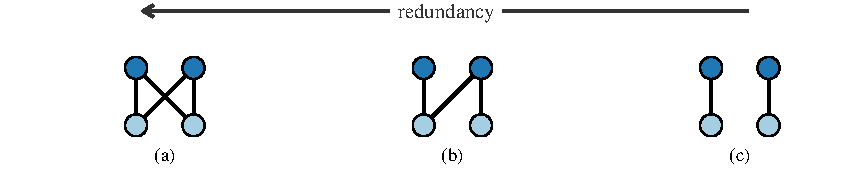
\includegraphics{motifs}
  \caption{
  \label{fig:motifs}
  Motifs are sub-networks that represent different patterns of interactions in ecological networks.
  Motifs can be seen as simple “building blocks” that show the underlying structure of the community and include different forms redundancy (generalisation/specialisation).
  The most redundant type of motifs in mutualistic networks is shown on the left and the least redundant on the right.
  }
\end{figure}

It has been shown that these structural groupings (compartments and motifs) can have important consequences for the stability and persistence of the communities \autocite{Neutel2002, Kondoh2008, Thebault2010, Stouffer2010, Stouffer2011}.
In food webs, for example, where most interactions are antagonistic, a high degree of compartmentalisation increases the persistence of the community by buffering the propagation of the effects of species extinctions beyond their compartment \autocite{Stouffer2011}.
Similarly, a food-web tri-trophic motif\footnote{A three species food chain with one producer, one consumer and one top predator} is more persistent in isolation than an omnivory motif\footnote{A three species web with one producer, one consumer and an omnivore that predates on the consumer and the primary producer}, however although less efficient by itself, the omnivory motif increases the persistence of the whole food web by a larger proportion \autocite{Stouffer2010}, perhaps because of the redundancy conferred by the omnivorous link.
This suggest that regardless if the ecological groups are structural or functional, consistent with the portfolio effect, redundancy within groups confers an insurance effect to the ecosystem \autocite{Walker1992}.

Here I propose to explicitly evaluate the effects that structural redundancy has in the stability of ecological networks.
Despite the clear positive implications of redundancy in overall stability, from a theoretical point of view it is expected to also have negative effects for individual species because it reduces the niche differentiation with its competitors.
Therefore I am interested in looking at the implications that redundancy has on both the conditions for stable coexistence (similar as in the previous section) and on the response of ecosystem to perturbations.
Because there are several ways to quantify the structural redundancy of a species, I aim to identify the redundancy that is most relevant to species coexistence and ultimately, ecosystem collapse.

In engineering, the reliability of a system is increased by making components that perform critical functions redundant.
Similarly in ecology, redundancy has been proposed to be a key factor contributing to the persistence of the ecosystem \autocite{Naeem1997,Naeem1998}.
There is both theoretical \autocite{Yachi1999} and empirical \autocite{Valone2008} evidence for the insurance hypothesis and, as mentioned, previous findings in food webs of antagonistic interactions support it.
However on pollination networks, where interactions are considered to be mutualistic, the effects of structural redundancy have not been thoroughly explored.
To date, only one study \autocite{Thebault2010} has explicitly looked at the effects of compartmentalisation on the stability of mutualistic networks.
Remarkably, contrary to what would be expected in an antagonistic system, some evidence suggest that compartmentalisation decreases both the persistence and resilience of mutualistic networks.
This might explain the fact that empirical mutualistic networks are in average less compartmentalised that their antagonistic counterparts \autocite{Thebault2010}.
But it does not explain why a large proportion of observed mutualistic networks are still significantly modular.

Previous theoretical work has largely assumed that the feedbacks of mutualistic interactions increase the growth rates of the focal species, while antagonistic interactions decrease it, which in turns allows the coexistence of a larger number of species (\autoref{fig:networks}) \autocite{Moeller2004, Bastolla2009}.
This assumption, however, ignores that in mutualistic systems, organisms might also compete to optimise the obtained benefits \autocite{Levin1970}.
Indeed evidence suggests that, in plant-pollinator systems, the increase of mutualistic interactions caused by invasive species does not translate into increased facilitation \autocite{Lopezaraiza-Mikel2007}.
Because plant reproduction depends strongly in the quality of the mutualistic service, mutualisms can be strongly altered when co-flowering species compete for the service of shared pollinators \autocite{Sargent2008, Mitchell2009}.
This happens because the visit of a pollinator does not lead to reproduction if pollen is transfered between different species of plants \autocite{Morales2008}.
Even though there are some mechanisms to mitigate the impacts of competition for mutualism and inter-specific pollen transfer \autocite{Waser1979, Ghazoul2006, Bartomeus2008a}, it has been found that invasive species, at high densities, are able to co-opt pollinators from native species \autocite{Pysek2011}, dominate the networks of pollen transport \autocite{Lopezaraiza-Mikel2007, Alarcon2010}, and ultimately decrease the seed output of native species \autocite{Munoz2008}.

Standard models of mutualism, which are used in both coexistence and collapse research, have so far only included intra-guild competition (for example competition for resources among plants) \autocite{Lever2014, Bastolla2009}, however stability attributes can change drastically if inter-guild interactions are not exclusively facilitative.
For instance, if only facilitation is taken into account, a fully connected and maximally redundant structure (left panel in \autoref{fig:networks} and \ref{fig:motifs}) represent the most favourable conditions for species coexistence and ecosystem collapse \autocite{Bastolla2009, Lever2014}.
On the other hand the same structure will be the undesirable if interactions were antagonistic because niche differentiation would be minimal \autocite{Stouffer2010}.

Although these standard models have been useful in recognising that all else being equal, a nested structure is indeed better than a random structure at facilitating biodiversity and delaying the onset of catastrophic collapses, they also predict that a maximally redundant network is better than the nested structure we tend to observe in nature (\autoref{fig:hypo_c2}).
My hypothesis is that competition for pollinators and its interplay with structural redundancy might be the key for explaining this discrepancy as well as the structural differences between mutualistic and antagonistic networks.

\begin{figure}[tbp]
  \centering
  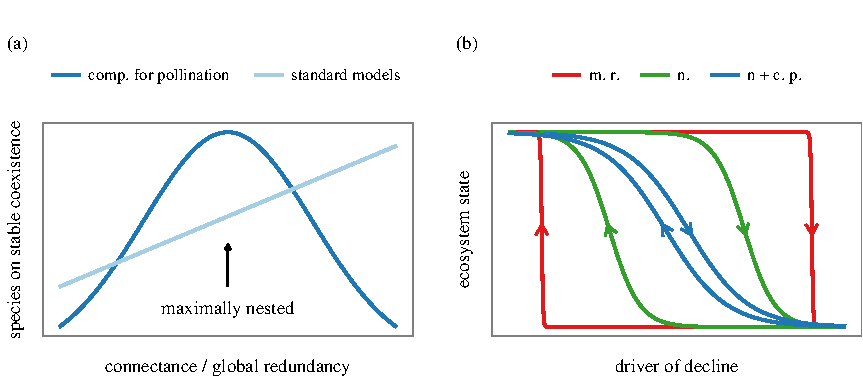
\includegraphics{hypo_c2}
  \caption{
  \label{fig:hypo_c2}
  (a) Standard models of mutualism predict a positive relationship between connectance (higher global redundancy) and biodiversity (light blue line), yet this is not observed in empirical communities. I argue that including competition-for-pollination will help explain why this orgy of facilitation is not observed in nature.
  Also, (b) standard models of pollination have found that a the more connected the network (red lines) the more it is resistant to drivers of decline; nested structures (green line) are also able to delay the onset of catastrophic declines more efficiently than random structures with no redundancy, the response to declines when competition for pollination is included (blue line) is however unknown.
  I predict that because plants that share pollinators are not exclusively facilitating each other, they do not collapse independently.
  Therefore decline should be more gradual and the hysteresis should be reduced.
  }
\end{figure}

I will use two approaches to evaluate this hypothesis.
In the first approach In the second approach I will take hand of motifs as an intuitive local metric of redundancy.
In a similar methodology as that used by Stouffer and Bascompte (2010) \autocite{Stouffer2010}, I will first evaluate the persistence of individual motifs (\autoref{fig:motifs}) with and without competition-for-pollinators when taken in isolation.
Then I will examine the relationship between the frequency with which those modules appear on empirical networks and the impact on the persistence of the pollination system.
I expect to

In the second approach I will extend the models developed in the previous section to explicitly include competition for pollinators.
Then I will construct a large number of synthetic networks of varied structure and numerically determine those that enable a large number of species to coexist (\hyperref[fig:hypo_c2]{Figure \ref{fig:hypo_c2}a}).
Also, I will explore the consequences that competition-for-pollinators has on delaying the onset of catastrophic collapse (\hyperref[fig:hypo_c2]{Figure \ref{fig:hypo_c2}b}).
I predict that the structure of ``optimal'' networks that include competition-for-pollinators is more consistent with the structure of networks observed on nature.
I argue that this empirical structure is the reflection of a balance between the redundancy required to maximise the facilitation effect of shared pollinators and minimise the competitive effects of interspecific pollen transfer.

Summing-up, I expect this research to help clarify the mechanisms that drive the structure of mutualistic networks.
While high redundancy might have biodiversity and stability benefits in mutualistic systems, it might also be responsible for the catastrophic collapses that occur once the perturbation has reached critical levels.
Ultimately we will be better positioned to understand why high diversity doesn't necessarily translate in higher redundancy \autocite{Bellwood2003b}.










\section{Controlling ecosystems for resilience management}

A plethora of empirical and theoretic evidence suggest that ecosystems have stable states on which self-organised processes and structures persist in equilibrium \autocite{Gunderson2000,Ives2007}.
However, disturbances, when large enough, can cause the ecosystem to move to a critical transition point.
When the ecosystem has reached this critical point, it can collapse, or more precisely, it can undergo a regime shift (a large, persistent transformation in ecosystem functioning and structure) after which the ecosystem enters an alternate stable state \autocite{Holling1973,May1976, Gunderson2000} (\hyperref[fig:critical_tran]{Figure \ref{fig:critical_tran}a}, \ref{fig:alt_ss}).


\begin{figure}[p]
  \centering
  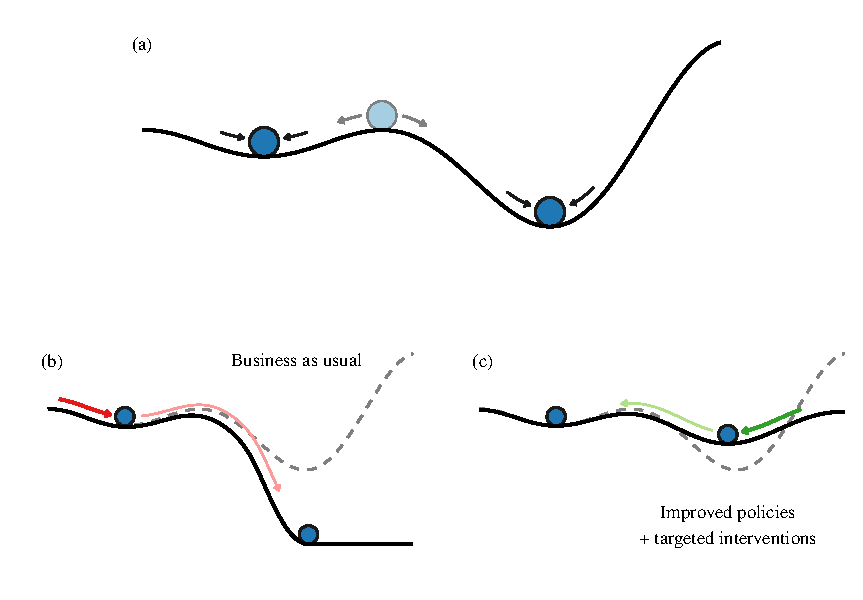
\includegraphics{critical_tran}
  \caption{
  \label{fig:critical_tran}
  Ecosystems tend to converge into stable states (dark blue circles).
  (a) After a small disturbance, the ecosystem is likely to return to the original stable state (black arrows) at a rate determined by its resilience (depicted in the figure as the slope of the curve).
  However, large disturbance (or a combination of smaller ones) can bring the ecosystem into a critical transition point (light blue) from which the ecosystem can undergo a regime shift and enter into an alternate stable state.
  Under a ``businness as usual'' scenario (b), the resilience of the desired state is diminished and human disturbances (red arrow) can push the ecosystem into an alternate stable state from which recovery is very difficult.
  By controlling the abundances of a set of key species (c), in theory, it is possible to induce a compensatory perturbation that weakens the resilience of the undesirable alternate stable state, and possibly push the ecosystem into recovery.
  }
\end{figure}

\begin{figure}[t]
    \centering
    \begin{subfigure}{0.47\textwidth}
        \centering
        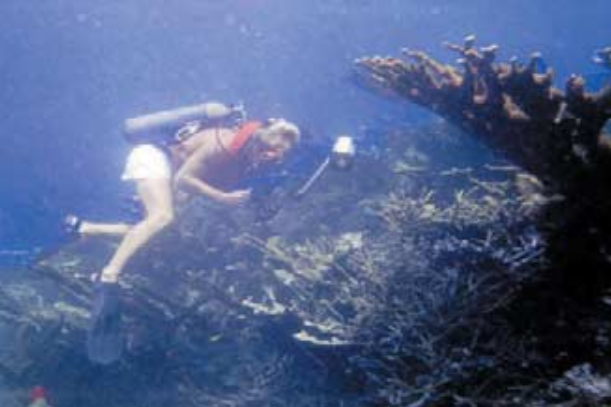
\includegraphics[width=\textwidth]{aas_before}
        \caption{Before}
    \end{subfigure}
    \hfill
    \begin{subfigure}{0.47\textwidth}
        \centering
        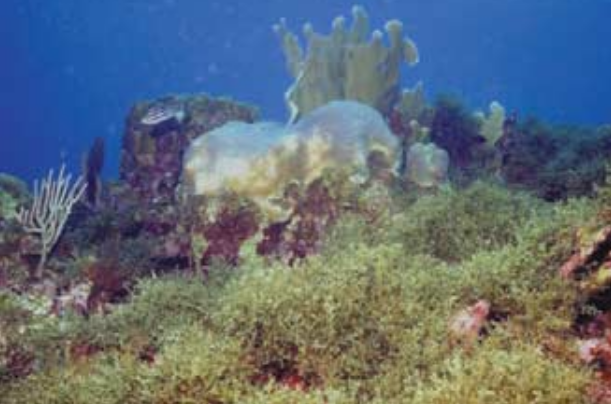
\includegraphics[width=\textwidth]{aas_after}
        \caption{After}
    \end{subfigure}
    \hfill
    \caption{
    One example of alternate states in tropical coral reefs, (a) assemblages dominated by corals in the Caribbean in 1979, and (b) the same reef, degraded and smothered by fleshy seaweed two decades later.
     By definition, regime shifts among alternate states constitute profound and often sudden changes in species composition, with major economic and social consequences. Reproduced from Hughes et al. 2005\autocite{Hughes2005}.
    }
    \label{fig:alt_ss}
\end{figure}

Often, ecosystems enter into these alternate stable states in response to anthropogenic pressures of global change like climate, invasive species, overexploitation or habitat loss (\hyperref[fig:critical_tran]{Figure \ref{fig:critical_tran}b}).
Unfortunately the frequency regime shifts is increasing, and this trend is likely to continue \autocite{Hughes2005}, which is severely compromising the provision of important ecosystem services we, and other species, strongly depend on \autocite{Hughes2013a}.
Some examples include the diminished production of fish after a food-web or habitat collapse in marine ecosystems \autocite{Hare2000, Daskalov2007, MacNeil2015}, or failure of crops after a collapse on pollination services \autocite{Pauw2007,Lever2014}.

As evidenced by the limited amount of success of restoration projects, bringing back ecosystems to a pre-disturbance state, or even to a more `desirable' state of ecosystem function, in which ecosystem services are somewhat recovered, is a particularly challenging endeavor \autocite{Graham2013a}.
So far we have only small-scale and localised examples of recovery \autocite{Carpenter2006a, Stockwell2009}, and in many cases the ecosystem fails to recover even after the disturbances that caused the regime shift are removed \autocite{Hughes2005}.
Moreover,some evidence suggest that recovery is at least partially determined by pre-disturbance structure of the community \autocite{Graham2015}, but we do not understand the mechanisms behind.
How to recover ecosystems from these undesirable alternate stable state is currently a major question in conservation and theoretical ecology.

The recovery of ecosystem depends strongly on the interactions between all species in the community and the dynamics that arise from these interactions.
Therefore, there have been calls to replace the predominant species-level approaches by ecosystem scale approaches to management and conservation.
However, perhaps with the exception of the mitigation of human-caused disturbances, ecosystem wide management can be expensive and difficult to attain.
Contrastingly, even though the efficacy of conservation measures directed to individual species can be argued, they are more intuitive, tractable, and usually easier to implement.

Unfortunately, we still do not understand how species-level interventions relate to the stability of the ecosystem as a whole.
This is important because it will allow us to determine if current interventions are indeed pushing the ecosystem to recovery or not.
Also, scaling the dynamics of individual species to the ecosystem level, will help to elucidate how to weaken the resilience of undesirable stable states, or strengthen the resilience of desirable states \autocite{Graham2013a}.
What is more, it will also help to determine if ecosystem recovery to a pre-disturbance state is possible and feasible from a management perspective.
Here, I propose to go one step beyond, and study the controllability of ecological networks and what network structures best support restoration efforts.

Ecosystems are challenging to control because they are large, complex, inhomogeneous, and non-linear systems.
However, recent work from theoretical physics has highlighted the possibility of regulating ecological networks by using targeted interventions in just some key species.
These species are not necessarily the most or least abundant, or invasive, but rather those that can drive the entire ecosystem dynamics \autocite{Liu2011} (\hyperref[fig:control_net]{Figure \ref{fig:control_net}a}).
By modifying the abundances of driver species, is in theory possible to control the state of the ecosystem, and possibly push the ecosystem into a pre-disturbance state or at least a more desirable alternate state of ecosystem function (\hyperref[fig:critical_tran]{Figure \ref{fig:critical_tran}c}, \hyperref[fig:control_net]{\ref{fig:control_net}b}).

\begin{figure}
  \centering
  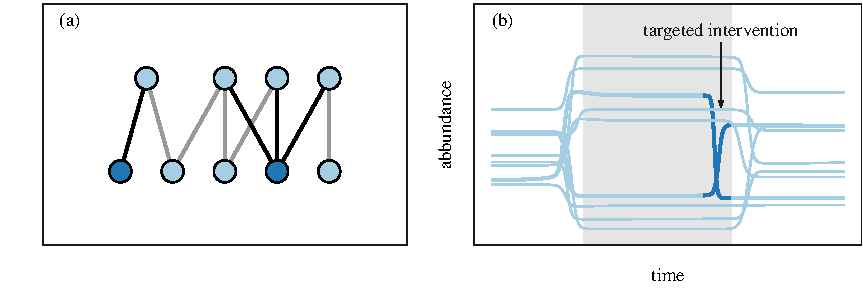
\includegraphics{control_net}
  \caption{
  \label{fig:control_net}
  In an ecological network, due to the interactions between species, changes in the abundances of any species are necessarily reflected in the abundances of their direct and indirect partners.
  (a) It is possible to find a minimal set of species (dark blue), such that the abundances of all other species (light blue) can be modified by interventions on the minimal set.
  If targeted interventions on those species are feasible (b), it is, in theory, possible to regulate the state of the ecosystem, and therefore reverse a regime shift that has lead an ecosystem into an alternate stable state (shaded area).
  }
\end{figure}

To achieve that, the first step is to determine the smallest possible set of driver species in which to apply conservation measures that modify their abundance \autocite{Liu2011, Isbell2013}.
I will determine these species by using `maximally matching' on the network of interactions---an algorithm that is already commonly used to find minimum sets in diverse areas of graph theory, image processing, and computational chemistry \autocite{Hopcroft1973,Neumann2010}.

By applying this framework to six pairs of invaded and uninvaded pollination networks \autocite{Bartomeus2008} I will examine the utility of this approach in a real world scenario.
Specifically I will explore the characteristics that make an species (such as the degree of generalisation or it's contribution to nestedness) more or less likely to function as a driver of ecosystem state, and whether these characteristics depend on the presence of an invasive species in the ecosystem.

The second step is to determine which interventions on the driver species are necessary to guide the ecosystem to the desired state.
Here I will use the subset of the population dynamics models developed for the previous research objective that show multiple alternate stable states.
I will then employ a recently developed algorithm that accounts for the non-linear dynamics present in ecological community \autocite{Cornelius2013, Cornelius2013a} to find the interventions that are necessary to modify ecosystem state.

However not all interventions are feasible; in reality, they are severely constrained by costs and scale.
For example, the an intuitive intervention to restore a coral reef from an algal dominated stable state (\hyperref[fig:alt_ss]{Figure \ref{fig:alt_ss}b}) to a coral dominated stable state (\hyperref[fig:alt_ss]{Figure \ref{fig:alt_ss}a}) is to simply decrease the abundance of fleshy seaweed and increase the abundance of stony corals.
This however is totally impractical; other interventions, for example those focused on species that predate on herbivore fishes, are more practical and might lead to similar results \autocite{Bennett2015}.
Therefore, I will focus on the feasible interventions that allow to modify the state of an ecosystem even when that state is not directly accessible.
These interventions are tailored on weakening the resilience of the undesirable state \autocite{Graham2013a, Standish2014a, Selkoe2015}.

Nevertheless, I anticipate to find empirical and simulated ecological communities in which none of the feasible interventions can lead to recovery to the original state.
In these cases, I will focus on exploring the implications of accepting a `novel ecosystem' \autocite{Hobbs2006}.
The concept of novel ecosystems highlights the possibility of an intermediate state, different from the original state, but one in which some ecosystem function and services have been restored \autocite{Graham2014a, Graham2015a}.
As pristine environments become less and less common, restoring some altered ecosystems back seems unrealistic under escalating anthropogenic pressures \autocite{Graham2015a}
Therefore I will find the interventions that maximise one ecosystem service, like pollination, while maintaining novel components in the ecosystem like invasive species.
Embracing change will ``allows conservation and management efforts to be directed more appropriately towards goals that are achievable''\autocite{Graham2014a}.


\begin{landscape}
\section{Research Plan}
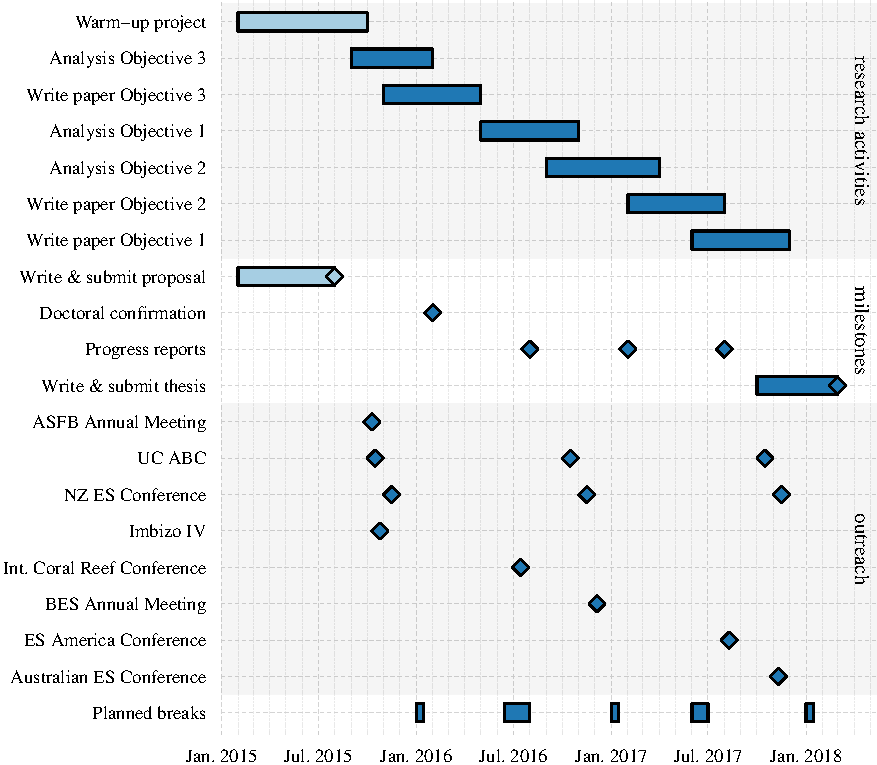
\includegraphics{schedule}
\end{landscape}

\printbibliography

\end{document}
